\documentclass[conference]{IEEEtran}
\IEEEoverridecommandlockouts
% The preceding line is only needed to identify funding in the first footnote. If that is unneeded, please comment it out.
%\usepackage{cite}
\usepackage{amsmath,amssymb,amsfonts}
\usepackage{algorithmic}
\usepackage{graphicx}
\usepackage{textcomp}
\usepackage{xcolor}
\usepackage{biblatex}
%\def\BibTeX{{\rm B\kern-.05em{\sc i\kern-.025em b}\kern-.08em
%    T\kern-.1667em\lower.7ex\hbox{E}\kern-.125emX}}
\addbibresource{presentation.bbl}
\begin{document}

\title{Edges to Handbags*}

\author{\IEEEauthorblockN{Zachary Harvey}
\IEEEauthorblockA{\textit{Computer \& Information Science Dept.} \\
\textit{SUNY Polytechnic Institute}\\
Utica, NY, USA \\
harveyz1@sunypoly.edu}
\and
\IEEEauthorblockN{Dr. Michael J. Reale}
\IEEEauthorblockA{\textit{Computer \& Information Science Dept.} \\
\textit{SUNY Polytechnic Institute}\\
Utica, NY, USA \\
realemj@sunypoly.edu}
}

\maketitle

\begin{abstract}
We are trying to build pictures of handbags from outlined drawings.
We build a pix2pix U-Net model to help accomplish this. We achived
marginal to good results for this with some very specific limits.
\end{abstract}

\begin{IEEEkeywords}
pix2pix, U-NET, outline, drawn
\end{IEEEkeywords}

\section{Introduction}
We are trying to build pictures of handbags from outline drawings. This proves to be
challenging because we have very little input in these drawings. This would enable designers
to be able to filter through ideas quickly. We tried using pix2pix and U-Net to accomplish this task.

\section{Related Work}
We are taking the core architecture from pix2pix \cite{imagetoimage}. The pix2pix
authors were able to achive decent results with their algorithms. There approaches were
very broad and we'd like to focus on a singular problem. There have been a couple of other
papers discussing this idea of outlines to objects. A group at MIT \cite{6247689} has
had good success with convert basic line drawings to geometric objects. The downside
is this work is really steered towards basic geometric shapes and not any organic soft shapes.
Zheng and Zhu have also showed other ways of reconstructing a 3D object from line drawing.
To decent success; however this to also looks to be towards mostly rigid bodied objects.


\section{Method}
We use a U-Net pix2pix architecture built in TensorFlow and Keras. The code for the
architecture was taken from the pix2pix tutorial on TensorFlows website \cite{pix2pix}.
We have eight steps down. Each step is sequential layer with a 2D convolution an optional
batch normalization which is only on the first layer. Then the output of the convolution is
pushed through a leaky relu. On the up side we have seven layers. Each layer is a sequential
with a 2D convolution transposed. We always apply a batch normalization. A dropout of 0.5 is
applied to the first three layers. The output is then pushed through a relu. I think we
insert skip connections but I odn't understand how those work. This creates our generator.
\par
The discriminator is much smaller. We take in the image generated by the generator. We run
it through three layers. Each layer is a sequential layer with a 2D convolution to an optional
normalization which is then passed through a leaky relu. The normalization is passed through
the last two layers. Once we're through those layers we pad out our data with zeros. Passing it
through another 2D convolution. Passing that through a batch normalization. Then we have a
leaky relu to more padding and finally another 2D convolution.
By using this method we were hoping to achieve at least a decent start to getting handbags.
We will use this as a jumping off point to get more complex handbags.
\subsection{Data}
The data is a setup into single images. Each image is width of 512 pixels with a
height of 256 pixels. This single images is two images paired together. The left side being
the outline of our handbag of size 256 by 256. The right side being a side profile of the
actual bag of size 256 by 256.


\section{Experiments}
We ran through the normal data set from the pix2pix \cite{imagetoimage} paper. We had mixed
results here.
\begin{figure}[h]
  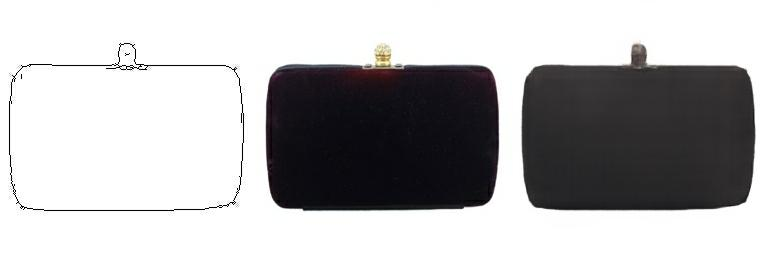
\includegraphics[width=0.5\textwidth]{./image_dump_39000.jpg}
  \caption{\label{fig:handbag39} Handbag after 39,000 steps}
  \centering
\end{figure}
The bag in figure \ref{fig:handbag39} had good results after 39,000 steps. The shape is there, the color
looks decent though it's lost the gold coloring. However this larger handbag in figure
\ref{fig:missing-data} had some problems. It appears as the algorithm is inventing the bottom of the bag
as the input drawing has left that out.
\begin{figure}[h]
  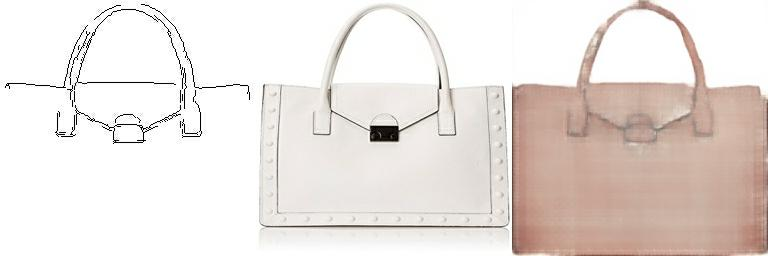
\includegraphics[width=0.5\textwidth]{./bad_result.jpg}
  \caption{\label{fig:missing-data} Input is missing data.}
  \centering
\end{figure}
So we decided to check against none square bags. We were hoping to see how the algorithm handled these instances.
This would hopeful help us lead to how it was handling input with missing data.
\begin{figure}[h]
  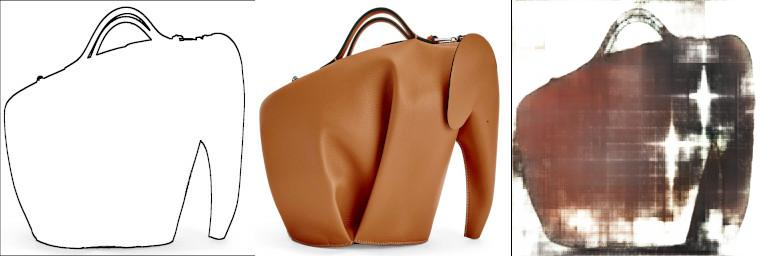
\includegraphics[width=0.5\textwidth]{./bad_elephant_33000.jpg}
  \caption{\label{fig:loewe} Loewe Elephant bag after 33,000 steps}
  \centering
\end{figure}
This bag built by Loewe is an elephant. We took a side profile and built an outline with GIMP. This image is after
33,000 steps. It looks like the algorithm is prefering to build square or rectanglar bags. It seems to ignore the
open space between the bag and the trunk of the elephant. 
\begin{figure}[h]
  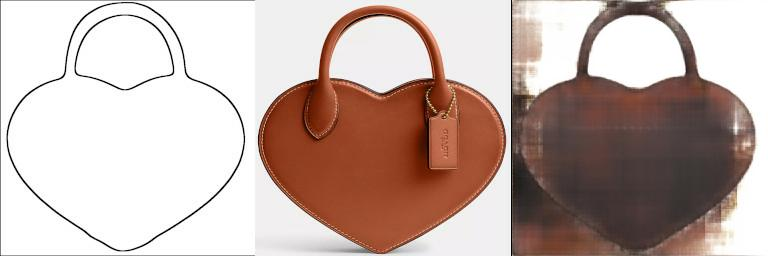
\includegraphics[width=0.5\textwidth]{./heart_33000.jpg}
  \caption{\label{fig:coach} Coachs Heart bag after 33,000 steps}
  \centering
\end{figure}
The Coach Heart bag in figure \label{fig:coach} also suggests that the algorithm favors square bags. 

\begin{figure}[h]
  \includegraphics[width=0.5\textwidth]{./imagetoimage_output.png}
  \caption{\label{fig:imagetoimage} Sample output from image to image paper \cite{imagetoimage}}
  \centering
\end{figure}
However Isola and Zhu \cite{imagetoimage} output appears to have cleaned up a lot of these results.
This suggests that maybe we did not train for long enough.

\section{Conclusion}


%\begin{figure}[p]
%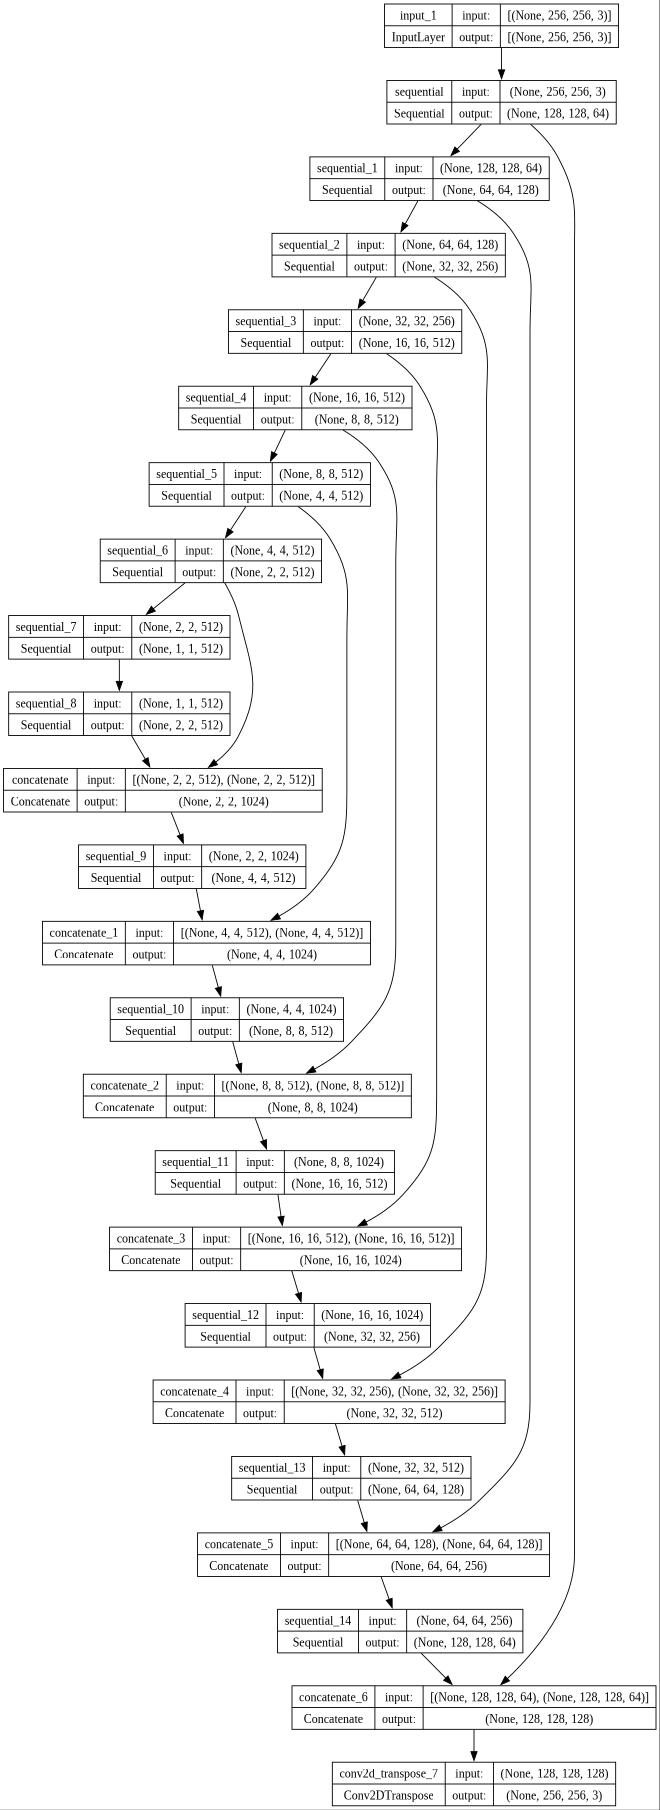
\includegraphics[scale=0.25]{./generator.jpg}
%\centering
%\end{figure}
%
%\begin{figure}[p]
%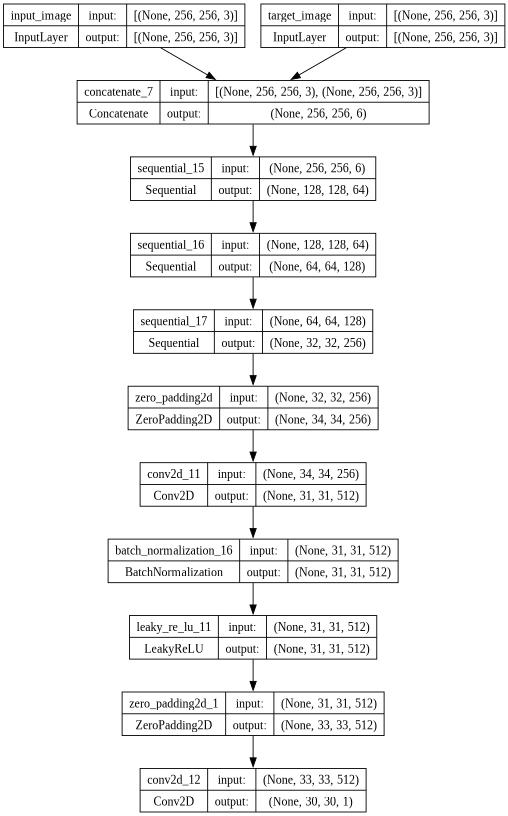
\includegraphics[width=0.38\textwidth]{./discriminator.jpg}
%\centering
%\end{figure}

\printbibliography
\end{document}
